
%(BEGIN_QUESTION)
% Copyright 2006, Tony R. Kuphaldt, released under the Creative Commons Attribution License (v 1.0)
% This means you may do almost anything with this work of mine, so long as you give me proper credit

De fleste AC-motordrifter modulerer spenningen til motoren proporsjonalt med frekvensen. Dette kalles volt-per-hertz-forholdet (V/Hz), og det konfigureres ofte som en konstant verdi over hele motorens driftsområde.

For å forstå hvorfor motorspenningen må moduleres proporsjonalt med frekvens når vi endrer hastigheten, er det nyttig å modellere den elektriske motoren som en enkel induktor (drevet av en AC-kilde med variabel spenning og variabel frekvens):

$$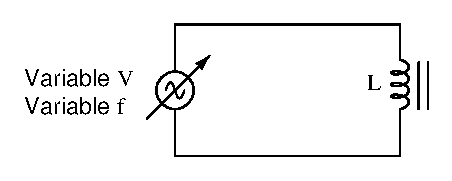
\includegraphics[width=15.5cm]{i01441x01.eps}$$

Hva vil skje med induktoren dersom vi reduserer AC-frekvensen mens AC-spenningen holdes konstant?

\underbar{file i01441}
%(END_QUESTION)





%(BEGIN_ANSWER)

Induktoren vil mest sannsynlig overopphetes og brenne opp. Når frekvensen synker, synker også den induktive reaktansen ($X_L$). Når reaktansen synker, blir motstanden i induktoren mot AC-strøm mindre, og strømmen øker tilsvarende. Denne økte strømmen vil overopphete induktoren (og også mette den magnetiske kjernen!). Derfor begrenser vi strømmen gjennom induktoren til normal verdi ved å redusere spenningen når vi reduserer frekvensen.

%(END_ANSWER)





%(BEGIN_NOTES)


%INDEX% Final Control Elements, motor: variable-speed (volts/hertz ratio)

%(END_NOTES)

